\begin{figure*}[!t]
    \centering
    
\includegraphics[width=\linewidth]{rtm_slope_pooled_2panel.png}
    \caption{\textbf{Baseline connectivity level predicts FC change in Sham but not Active tFUS.} (a) Sham tFUS: subject-level scatter of baseline sgACC FC (x-axis) versus change from baseline $\Delta\mathrm{FC}=\mathrm{FC}_{t}-\mathrm{FC}{\mathrm{pre}}$ (y-axis), with data pooled across tFUS $(\circ)$ and post-sonication $(\triangle)$ windows. The regression line is derived from an OLS model with fixed effects for subject, time-window, and condition. The inverse relationship between $\Delta$ FC and baseline FC observed in the Sham condition is consistent with a regression-to-the-mean account. 
    (b) Same as (a) but now shown for Active tFUS. The slope of the regression line is mildly positive and does not differ significantly from zero. Importantly, the difference in slopes between Active and Sham is significant ($p=0.013$), indicating that baseline effects are not driving the observed post-sonication connectivity increase during Active stimulation.}
    \label{fig:rtm_slope_pooled_2panel}
\end{figure*}

\subsection*{Increased sgACC-whole-brain connectivity after Active tFUS}
\noindent 
To formally test whether tFUS modulated sgACC-centered connectivity beyond Sham, we fit a subject-level linear mixed-effects model. For each subject, condition (Sham, Active), and time window (Pre, tFUS, Post), we computed the mean FC between the sgACC and all other atlas parcels (1023), yielding one sgACC--whole-brain FC value per subject-time-condition (16 subjects $\times$ 2 conditions $\times$ 3 time windows $=$ 96 observations). Time window and condition were modeled as categorical fixed effects with \textit{Pre} and \textit{Sham} as reference levels, and a random intercept for subject accounted for repeated measures. This parameterization allowed us to directly test whether the change in sgACC FC from Pre to Post (and from Pre to tFUS) differed between Active and Sham sessions (time$\times$condition interaction).

The results of the model are presented in Table~\ref{tab:mixedlm_sgacc}. Within the Sham condition, sgACC FC did not change reliably over time (tFUS vs.\ Pre: $\beta = -0.020$, $p = 0.444$; Post vs.\ Pre: $\beta = -0.011$, $p = 0.671$), indicating a lack of systematic drift in sgACC-centered FC. Importantly, the post-sonication time$\times$condition interaction was significant: the additional Pre-to-Post change in the Active session relative to Sham was positive ($\beta = 0.079$, 95\% CI $[0.006,0.151]$, $p = 0.033$), indicating a significant enhancement of sgACC FC. The corresponding interaction at the tFUS window showed a similar but nonsignificant tendency ($\beta = 0.060$, $p = 0.104$). Together, these results support a conservative but robust conclusion that Active tFUS to the sgACC is associated with increased post-sonication connectivity. 

These subject-level effects are visualized for Sham and Active sessions in Fig.~\ref{fig:sgacc_violin_2panel}. In the Sham condition (Fig.~\ref{fig:sgacc_violin_2panel}a), sgACC FC exhibits no systematic monotonic change from Pre to tFUS to Post, and individual trajectories fluctuate around a stable mean. In contrast, the Active tFUS condition (Fig.~\ref{fig:sgacc_violin_2panel}b) shows a clear ``ramping'' pattern: sgACC FC increases from a lower baseline to higher values during tFUS and reaches its highest levels post-sonication. The alignment of individual trajectories with the model-based interaction effect visually reinforces the conclusion that tFUS strengthens connectivity with the sgACC in a manner that outlasts the stimulation.

Panels c–d plot baseline-referenced changes ($\Delta\mathrm{FC}=\mathrm{FC}_t-\mathrm{FC}_{\mathrm{pre}}$) for the tFUS and post-sonication windows, respectively. Sham values remain centered near zero across windows, whereas the FC change with Active stimulation is positive both during and after stimulation. A planned post-hoc contrast of $\Delta\mathrm{FC}$ between Active and Sham indicated a borderline significant trend during the tFUS window (Active–Sham $\Delta\mathrm{FC}=+0.060$; $p=0.051$) and a significant effect post-sonication (Active–Sham $\Delta\mathrm{FC}=+0.079$; $p=0.034$). 

\begin{table*}[t]
    \centering
    \caption{\textbf{Linear mixed-effects model of subject-level mean sgACC FC.}
    The dependent variable is the mean sgACC--whole-brain FC for each subject, condition, 
    and time window. Time window (Pre, tFUS, Post) and condition (Sham, Active) are coded 
    categorically with \textit{Pre} and \textit{Sham} as reference levels. The model includes 
    a random intercept for subject. The key effect of interest is the post-sonication 
    time~$\times$~condition interaction, indicating a larger Pre-to-Post increase in sgACC FC 
    for Active tFUS relative to Sham.}
    \label{tab:mixedlm_sgacc}
    \begin{tabular}{lccccc}
    \toprule
    Effect & Estimate & SE & $z$ & $p$-value & 95\% CI \\
    \midrule
    Intercept (Sham, Pre)                                       & 0.121 & 0.021 &  5.89 & $<0.001$ & [0.081,\ 0.161] \\
    Time: tFUS vs.\ Pre (Sham)                                  &-0.020 & 0.026 & -0.77 & 0.444   & [-0.071,\ 0.031] \\
    Time: Post vs.\ Pre (Sham)                                 &-0.011 & 0.026 & -0.42 & 0.671   & [-0.062,\ 0.040] \\
    Condition: Active vs.\ Sham (at Pre)                       &-0.061 & 0.026 & -2.34 & 0.019   & [-0.112,\ -0.010] \\
    Interaction: (tFUS vs.\ Pre) $\times$ (Active vs.\ Sham)    & 0.060 & 0.037 &  1.63 & 0.104   & [-0.012,\ 0.133] \\
    \bf{Interaction: (Post vs.\ Pre) $\times$ (Active vs.\ Sham)}  & \bf{0.079} & \bf{0.037} &  \bf{2.13} & \bf{0.033}   & \bf{ [0.006,\ 0.151] } \\
    \midrule
    Subject random intercept variance                          & 0.001 &       &       &         &              \\
    Residual variance                                          & 0.0055&       &       &         &              \\
    \bottomrule
    \end{tabular}
    \end{table*}



        
        \subsection*{Baseline connectivity level predicts FC change in Sham but not Active tFUS.}
        \noindent
        Due to the different baseline FC values between Sham and Active sessions, it was important to rule out that discrepancies in baseline level drive the observed post-sonication connectivity increase (a ``regression-to-the-mean'' effect). To address this, we modeled the change from baseline ($\Delta FC$) as the dependent variable using OLS with fixed effects for subject, time window, condition, and baseline FC, as well as an interaction term between baseline and condition. 

        The model explained substantial variance in $\Delta \mathrm{FC}$ ($R^2=0.676$; $p=0.017$). In Sham, higher baseline sgACC FC predicted larger subsequent decreases in connectivity (slope $=-0.776$, $95\%$ CI $[-1.37,-0.18]$, $p=0.010$; Table \ref{tab:rtm_slope_pooled}), consistent with a regression-to-the-mean account. In the Active condition, however, the baseline--change association did not significantly differ from zero (slope $+0.207$, $95\%$ CI $[-0.575,\,0.989]$, n.s.). Critically, the slope difference between conditions was significant ($\beta_3=+0.983$, 95\% CI $[0.203,\,1.763]$, $p=0.013$), indicating that the mapping from baseline to subsequent change differs under stimulation. Figure~\ref{fig:rtm_slope_pooled_2panel} shows the relationship between baseline connectivity and subsequent FC change (circle markers denote the tFUS window, triangles denote the post-sonication window). The inverse relationship between baseline level and FC difference is evident for Sham (Panel a), while the slope of the regression line is mildly positive in the Active condition (Panel b).


    
        \begin{table*}[t]
            \centering
            \caption{\textbf{Testing the relationship between baseline FC and the subsequent change in connectivity (``Baseline--change slope test'').} We fit an ordinary least squares model with fixed effects for subject, time-window (categorical with tFUS reference), condition (categorical with Sham reference), and baseline FC (z-scored). The dependent variable is $\Delta \mathrm{FC}_{ict} = \mathrm{FC}_{ict} - \mathrm{FC}_{ic,\mathrm{pre}}$ for subject $i$, condition $c$ and time window $t$. We assay whether the baseline--change slopes are significantly different between Sham and Active.}
            \label{tab:rtm_slope_pooled}
            \setlength{\tabcolsep}{10pt}
            \begin{tabular}{lccc}
            \toprule
            \textbf{Term} & \textbf{Estimate} & \textbf{95\% CI} & \textbf{$p$} \\
            \midrule
            Sham slope $\big(\partial\,\Delta\mathrm{FC}/\partial\,\mathrm{FC}_{\text{pre}}\big)$
            & $-0.776$ & $[-1.370,\,-0.182]$ & $0.010$ \\
            Active slope $\big(\partial\,\Delta\mathrm{FC}/\partial\,\mathrm{FC}_{\text{pre}}\big)$
            & $+0.207$ & $[-0.575,\,0.989]$ & n.s. \\
            \addlinespace[2pt]
            \textbf{Slope difference (Active $-$ Sham)} & \textbf{+0.983} & \textbf{[0.203,\,1.763]} & \textbf{0.013} \\
            \midrule
            $R^2$ & $0.676$ & & \\
            $N$ (rows) & $64$ & & \\
            Clusters (subjects) & $16$ & & \\
            \bottomrule
            \multicolumn{4}{p{0.9\linewidth}}{\footnotesize
            \textit{Model.}
            $\Delta \mathrm{FC}_{ict}
            = \alpha_i
            + \gamma\,\mathbb{I}[t=\mathrm{post}]
            + \beta_1\,\widetilde{\mathrm{FC}}_{ic,\mathrm{pre}}
            + \beta_2\,\mathbb{I}[c=\mathrm{active}]
            + \beta_3\,\widetilde{\mathrm{FC}}_{ic,\mathrm{pre}}\times \mathbb{I}[c=\mathrm{active}]
            + \varepsilon_{ict}$,
            with subject fixed effects $\alpha_i$, time-window fixed effect $\gamma$ (tFUS reference), baseline FC fixed effect $\beta_1$, condition fixed effect $\beta_2$, and baseline-condition interaction $\beta_3$.
            The baseline $\widetilde{\mathrm{FC}}_{ic,\mathrm{pre}}$ is mean-centered.
            The ``Active slope'' is the linear combination $\beta_1+\beta_3$; the ``Slope difference'' tests $H_0\!:\beta_3=0$.
            Observations: $16$ subjects $\times$ $2$ conditions $\times$ $2$ windows $=64$.}
            \end{tabular}
            \end{table*}

        \begin{figure*}[!t]
            \centering
            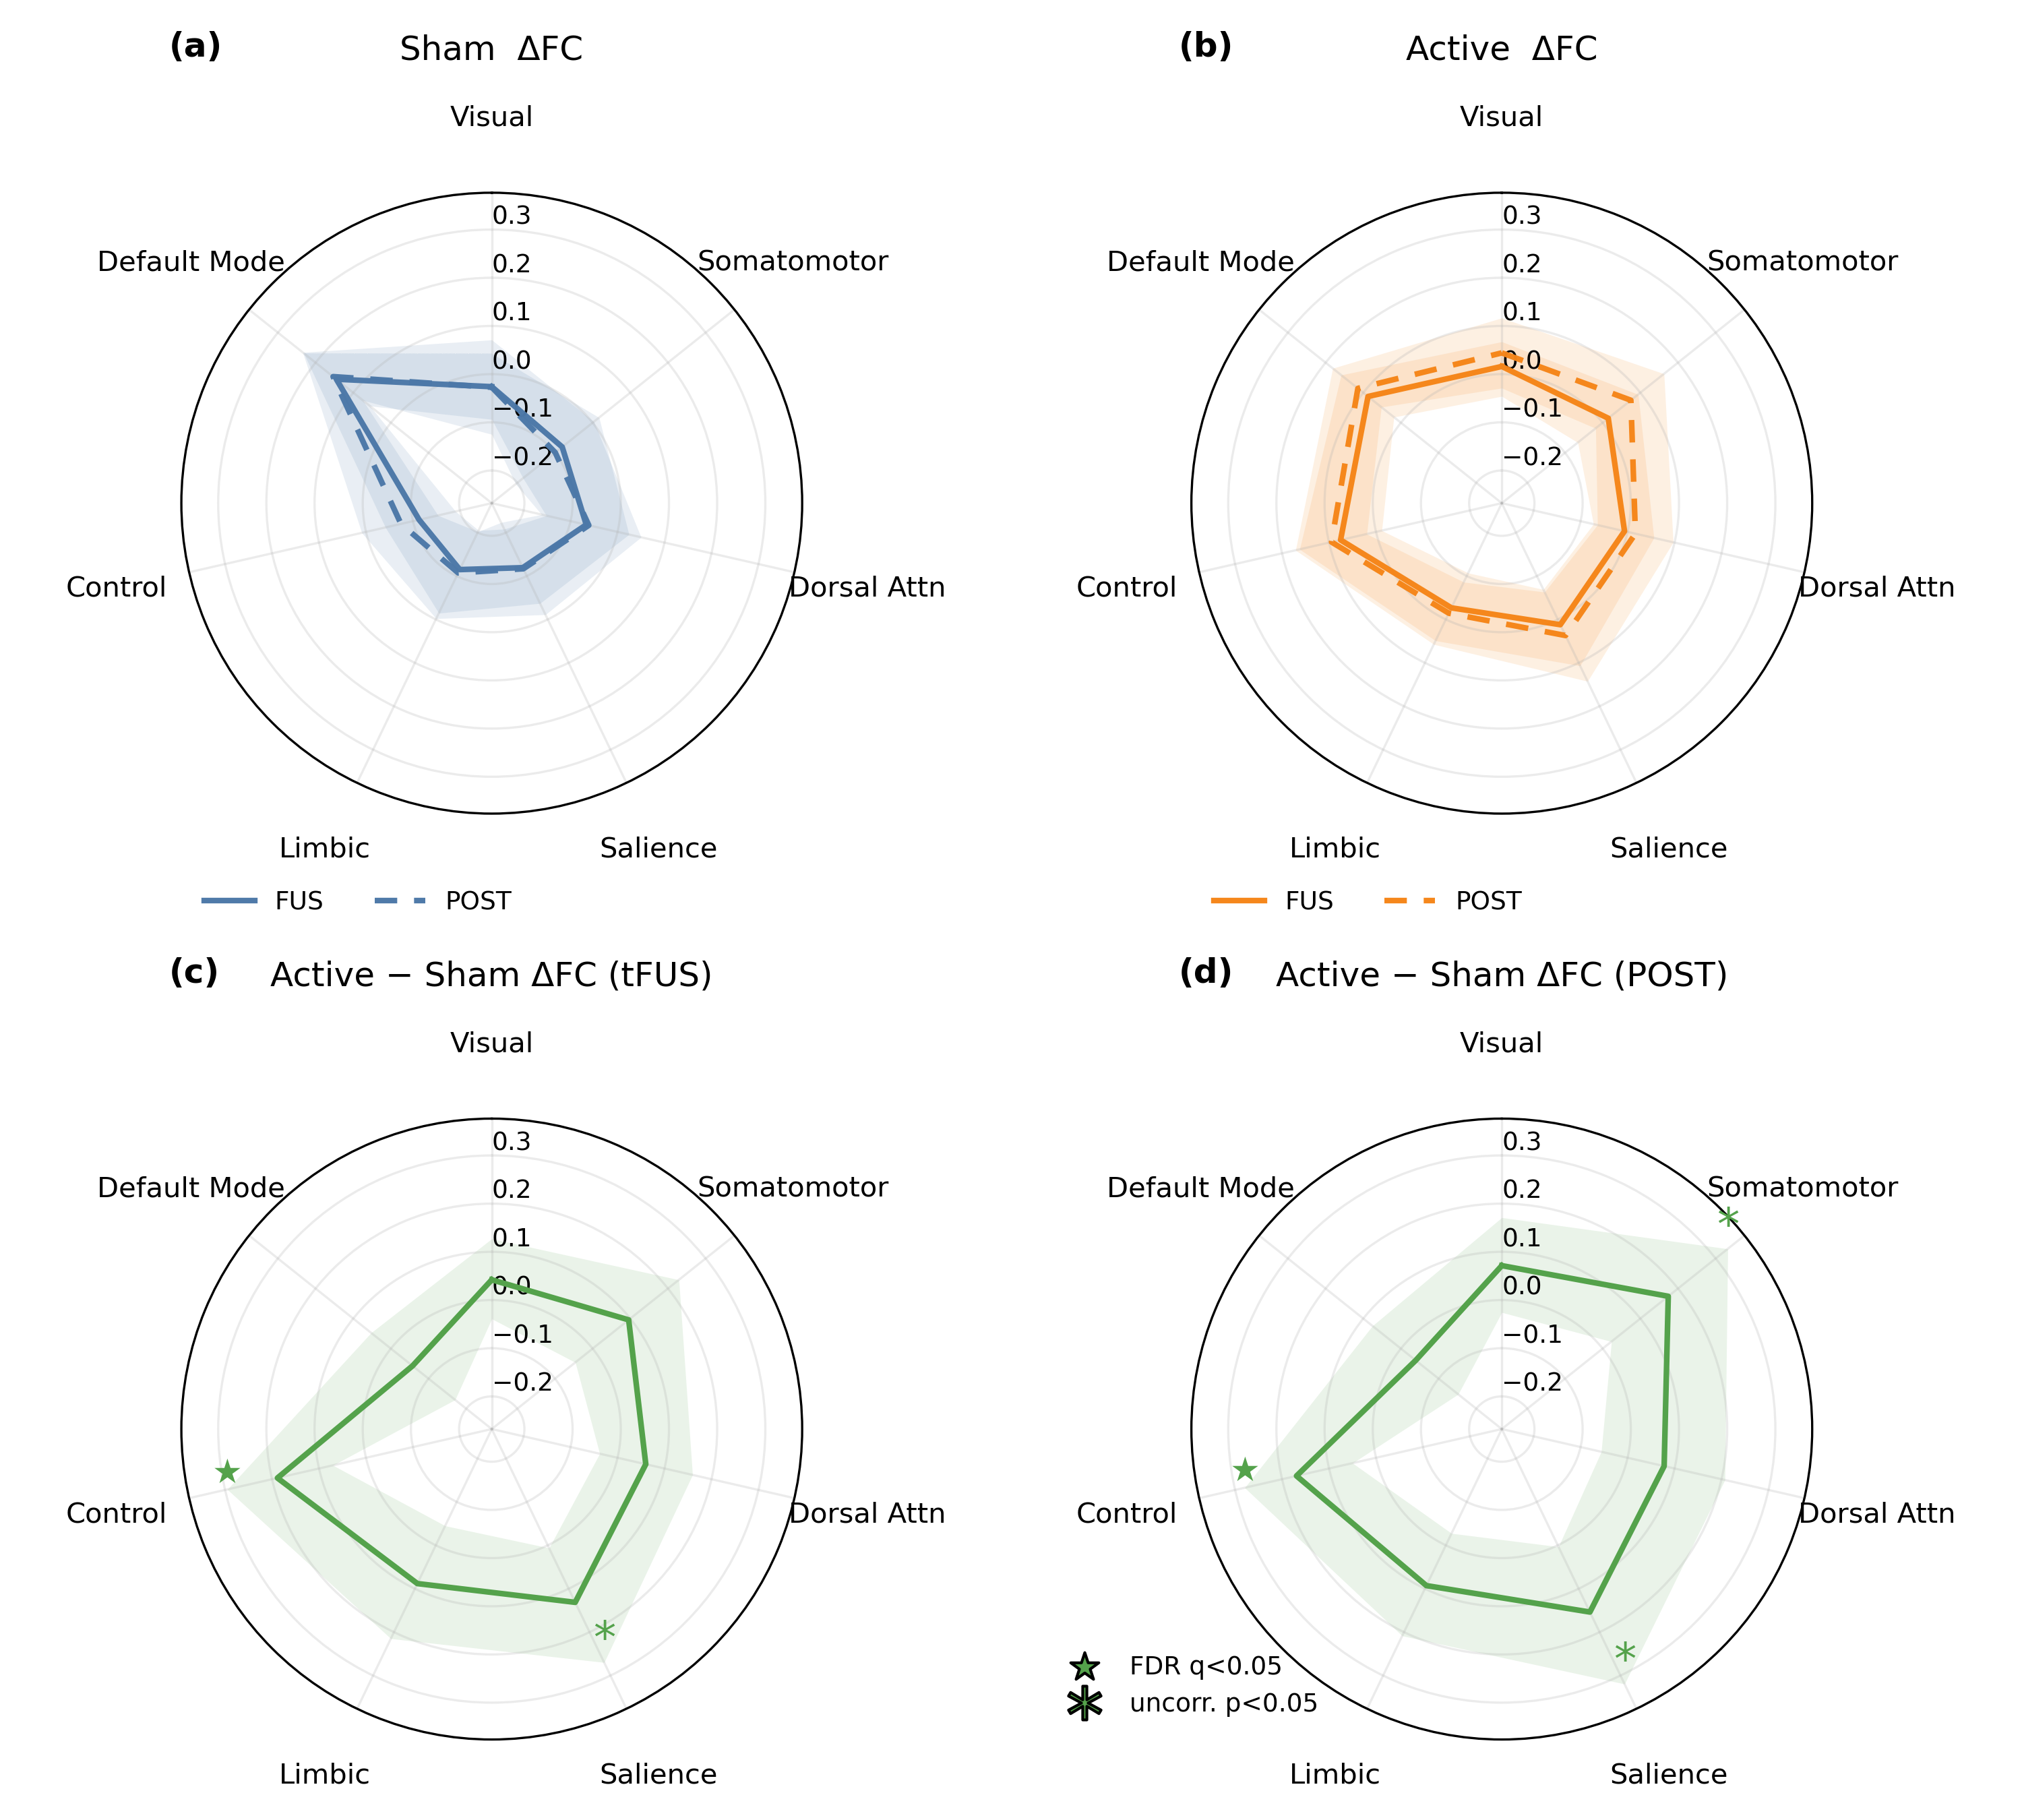
\includegraphics[width=\linewidth]{network_level_specificity_polar.png}
            \caption{\textbf{Network specificity of the sgACC connectivity increase under Active tFUS.}
            (a) \emph{Sham sessions:} baseline-referenced changes ($\Delta$FC) in sgACC coupling with the Yeo-7 networks indicate that the sgACC's connectivity with the Default Mode Network (DMN) increases over the course of the 15 minute recording (\texttt{tFUS}: solid; \texttt{Post}: dashed). 
            (b) \emph{Active tFUS:} In contrast, $\Delta$FC exhibits a more uniform pattern across the 7 canonical networks, with the largest increase observed at the Cognitive Control network.
            (c--d) \emph{Active--Sham differences in $\Delta$FC} shown at \texttt{tFUS} (c) and \texttt{Post} (d). Symbols mark directional tests ($H_1:\ \Delta\mathrm{FC}_{\text{active}}>\Delta\mathrm{FC}_{\text{sham}}$) corrected across networks using FDR: 
            filled star \raisebox{0.2ex}{\scriptsize$\star$}, $q<0.05$; asterisk \raisebox{0.2ex}{\scriptsize*}, uncorrected $p<0.05$. 
            At \texttt{tFUS}, the Cognitive Control network's coupling with the sgACC is significantly positive (FDR $q=0.028$), with the Salience network showing a positive trend (uncorr.\ $p=0.026$, $q=0.077$). 
            At \texttt{Post}, the Cognitive Control network's coupling remains elevated ($q=0.028$), while the Salience and Somatomotor networks exhibit trend-level, positive differences (Salience $q=0.077$; Somatomotor $q=0.066$). This data is consistent with a redistribution of sgACC coupling from the DMN toward task-positive networks (Control, Salience, Somatomotor) under Active stimulation.}
            \label{fig:network_level_specificity}
        \end{figure*}



    \subsection*{Network-level redistribution of sgACC connectivity.}
    \noindent
    Having confirmed a post-sonication increase in sgACC connectivity under Active stimulation, we next examined which large-scale networks expressed this additional coupling. Using the Yeo-7 parcellation \cite{yeo2011organization} (Visual, Cognitive Control, Default Mode, Dorsal Attention, Limbic, Salience, and Somatomotor networks), we compared subject-level baseline-referenced $\Delta$FC at the tFUS and Post time windows (summarized in Table~\ref{tab:network_specificity_onesided}). A clear dissociation emerged: in \emph{Sham}, increases from baseline were confined to the Default Mode Network (DMN), whereas in \emph{Active}, sgACC exhibited distributed increases to multiple non-DMN networks during and after sonication (Fig.~\ref{fig:network_level_specificity}). The Cognitive Control network showed the largest Active--Sham differences ($\Delta\mathrm{FC} = +0.19$ at tFUS and $+0.17$ at Post; nominal $p=0.0024$ and $0.0040$, FDR-adjusted $q=0.028$ for both; Table~\ref{tab:network_specificity_onesided}). Positive, albeit smaller, Active--Sham differences were also observed for Visual ($+0.042$ at tFUS; $+0.071$ at Post), Somatomotor ($+0.096$ at tFUS; $+0.174$ at Post; $q_{\mathrm{FDR}}=0.066$), Salience ($+0.131$ at tFUS; $+0.154$ at Post; $q_{\mathrm{FDR}}=0.077$), Dorsal Attention ($+0.060$ at tFUS; $+0.078$ at Post), and Limbic ($+0.088$ at tFUS; $+0.093$ at Post) networks. In contrast, the DMN showed the opposite polarity (Active--Sham $\Delta\mathrm{FC}=-0.057$ at tFUS; $-0.039$ at Post). 

    %Symbols: \textsuperscript{$\star$} $q<0.05$; \textsuperscript{$\dagger$} $q<0.10$; \textsuperscript{*} uncorrected $p<0.05$.
    \begin{table*}[t]
        \centering
        \caption{\textbf{Network-specific tests of Active--Sham differences in baseline-referenced $\Delta$FC.}
        One-sided hypotheses $H_1:\ \Delta\mathrm{FC}_{\text{active}}>\Delta\mathrm{FC}_{\text{sham}}$ were evaluated per network and window; $p$ values are one-sided and FDR corrected within the family of network\,$\times$\,window tests (\emph{q}). }
        \label{tab:network_specificity_onesided}
        \setlength{\tabcolsep}{6pt}
        \begin{tabular}{l l c c r r r}
        \toprule
        Network & Window & $n_{\mathrm{sham}}$ & $n_{\mathrm{active}}$ & $t$ & $p$ & $q_{\mathrm{FDR}}$ \\
        \midrule
        Visual           & tFUS & 16 & 16 &  0.884 & 0.187 & 0.219 \\
        Visual           & Post & 16 & 16 &  1.129 & 0.132 & 0.193 \\
        \textbf{Control}          & \textbf{tFUS} & \textbf{16} & \textbf{16} &  \textbf{3.139} & \textbf{0.0024} & \textbf{0.028} \\
        \textbf{Control}          & \textbf{Post} & \textbf{16} & \textbf{16} &  \textbf{2.860} & \textbf{0.0040} & \textbf{0.028} \\
        Default Mode     & tFUS & 16 & 16 & -0.961 & 0.834 & 0.834 \\
        Default Mode     & Post & 16 & 16 & -0.722 & 0.765 & 0.823 \\
        Dorsal Attention & tFUS & 16 & 16 &  1.036 & 0.155 & 0.198 \\
        Dorsal Attention & Post & 16 & 16 &  1.103 & 0.138 & 0.193 \\
        Limbic           & tFUS & 16 & 16 &  1.345 & 0.093 & 0.163 \\
        Limbic           & Post & 16 & 16 &  1.445 & 0.078 & 0.163 \\
        \textbf{Salience}         & \textbf{tFUS} & \textbf{16} & \textbf{16} &  \textbf{2.042} & \textbf{0.026} & \textbf{0.077}\\
        \textbf{Salience}         & \textbf{Post} & \textbf{16} & \textbf{16} &  \textbf{1.958} & \textbf{0.028} & \textbf{0.077}\\
        Somatomotor    & tFUS & 16 & 16 &  1.413 & 0.085 & 0.163 \\
        \textbf{Somatomotor}      & \textbf{Post} & \textbf{16} & \textbf{16} &  \textbf{2.328} & \textbf{0.014} & \textbf{0.066} \\
        \bottomrule
        \end{tabular}
        \end{table*}




\subsection*{Examining the influence of distance-to-target on FC changes.}
\noindent
Due to individual differences in head geometry, the distance from the transducer to the sgACC varied across our cohort (58 $\pm$ 5 mm). The transducer's fixed beampattern meant that the intensity of stimulation at the target also varied between subjects, and we asked whether this could explain inter-individual variability in observed FC changes. We thus measured the scalp--to--sgACC distance for each subject, and then correlated the result with the FC change using a mixed-effects model (Table \ref{tab:distance_moderation_mixedlm}).

In the \emph{Sham} condition, the slope of FC per 1 SD of distance was slightly positive (Pre: $+0.014$; tFUS: $+0.027$; Post: $+0.030$). In the \emph{Active} condition, the slope was near zero to negative (Pre: $+0.002$; tFUS: $-0.004$; Post: $-0.013$). The derived distance-slope difference in the Post time window (Active $-$ Sham) was $-0.043$ per 1 SD ($= -0.074$ per 10 mm, SE $=0.025$, $z=-1.73$, $p=0.083$), indicating a \emph{trend} toward attenuation of the FC increase with greater distance-to-target. Importantly, the principal time$\times$condition contrast in the Post time window remained significant after including distance ($\beta=+0.079$, $p=0.024$), demonstrating that the main stimulation effect is robust to anatomical distance. Figure ~\ref{fig:distance_loess} depicts the relationship between scalp--to--sgACC distance and change in FC during (a) and after (b) tFUS. Interestingly, application of the Locally Estimated Scatterplot Smoothing (LOESS) technique is suggestive of an inverted U-shaped curve, potentially hinting at the maximization of effects for subjects whose sgACC coincides with the transducer's focus. 


\begin{table*}[t]
    \centering
    \small
    \caption{\textbf{Moderation of tFUS effects on sgACC connectivity by scalp-to-sgACC distance}. 
Fixed effects included time window (reference = Pre), condition (reference = Sham), z-scored scalp–to–sgACC distance ($\mathrm{distance}_z$; one SD $\approx$ 5\,mm across participants), all two-way interactions (time$\times$condition, time$\times$distance, condition$\times$distance), and the three-way time$\times$condition$\times$distance interaction. A subject-specific random intercept modeled baseline differences. Models were fit by maximum likelihood; Wald $z$-tests (two-sided, $\alpha=0.05$) are reported for fixed effects. Positive coefficients indicate higher sgACC–whole-brain FC. The Post$\times$Active term corresponds to the difference-in-differences contrast (Active vs.\ Sham in the Pre$\rightarrow$Post change), and the Post$\times$Active$\times\mathrm{distance}_z$ term tests whether that effect varies with distance.}
    \label{tab:distance_moderation_mixedlm}
    \setlength{\tabcolsep}{8pt}
    \begin{tabular}{lccccc}
    \toprule
    \textbf{Effect} & \textbf{Estimate} & \textbf{SE} & \textbf{$z$} & \textbf{$p$} & \textbf{95\% CI} \\
    \midrule
    Intercept (Sham, Pre)                                             & 0.121 & 0.019 &  6.242 & $<\!0.001$ & [0.083,\ 0.159] \\
    Time: tFUS vs.\ Pre (Sham)                                       &-0.020 & 0.025 & -0.814 & 0.416      & [-0.068,\ 0.028] \\
    Time: Post vs.\ Pre (Sham)                                       &-0.011 & 0.025 & -0.451 & 0.652      & [-0.059,\ 0.037] \\
    Condition: Active vs.\ Sham (at Pre)                             &-0.061 & 0.025 & -2.485 & 0.013      & [-0.109,\ -0.013] \\
    Time$\times$Condition: (tFUS vs.\ Pre)$\times$(Active vs.\ Sham) & 0.060 & 0.035 &  1.731 & 0.083      & [-0.008,\ 0.128] \\
    \textbf{Time$\times$Condition: (Post vs.\ Pre)$\times$(Active vs.\ Sham)} & \textbf{0.079} & \textbf{0.035} &  \textbf{2.261} & \textbf{0.024}      & \textbf{[0.010,\ 0.147]} \\
    \addlinespace[3pt]
    Distance ($\mathrm{distance}_z$)                                  & 0.014 & 0.019 &  0.730 & 0.466      & [-0.024,\ 0.052] \\
    Time$\times$Distance: (tFUS vs.\ Pre)$\times \mathrm{distance}_z$ & 0.012 & 0.025 &  0.504 & 0.614      & [-0.036,\ 0.061] \\
    Time$\times$Distance: (post vs.\ Pre)$\times \mathrm{distance}_z$ & 0.016 & 0.025 &  0.639 & 0.523      & [-0.032,\ 0.064] \\
    Condition$\times$Distance: (Active vs.\ Sham)$\times \mathrm{distance}_z$ & -0.012 & 0.025 & -0.501 & 0.617 & [-0.060,\ 0.036] \\
    Time$\times$Condition$\times$Distance: (tFUS vs.\ Pre)$\times$(Active vs.\ Sham)$\times \mathrm{distance}_z$ & -0.018 & 0.035 & -0.520 & 0.603 & [-0.086,\ 0.050] \\
    Time$\times$Condition$\times$Distance: (Post vs.\ Pre)$\times$(Active vs.\ Sham)$\times \mathrm{distance}_z$ & -0.030 & 0.035 & -0.872 & 0.383 & [-0.098,\ 0.038] \\
    \midrule
    \multicolumn{6}{l}{\textit{Derived contrast (distance-slope difference at Post, Active$-$Sham):}} \\
    \multicolumn{1}{l}{\hspace{1em}$\lambda + \kappa_{\mathrm{post}}$ (per 1 SD)} & \multicolumn{1}{c}{ -0.043} & 0.025 & -1.73 & 0.083 & [-0.092,\ 0.006] \\
    %\midrule
    %Subject random intercept variance                                 & 0.001 &       &       &       &               \\
   % Residual variance (Scale)                                         & 0.0048&       &       &       &               \\
   % \midrule
   % $N$ (rows) & \multicolumn{5}{l}{96 \quad (16 subjects $\times$ 2 conditions $\times$ 3 windows)} \\
   % Log-likelihood & \multicolumn{5}{l}{112.4805 \quad\quad Converged: Yes} \\
    \bottomrule
    \end{tabular}
    
    \vspace{4pt}
\footnotesize\textit{Notes.} Reference levels: time = Pre; condition = Sham. $\mathrm{distance}_z$ is z-scored
(distance mean $=58$\,mm; SD $=5$\,mm), so coefficients on $\mathrm{distance}_z$ and any interaction
thereof are interpreted \emph{per 1 SD of distance}. The key time$\times$condition
effect at Post remains significant after including distance (estimate $=0.079$, $p=0.024$), indicating robustness of the
main stimulation effect to anatomical distance.
\end{table*}
\begin{figure*}[!t]
    \centering
    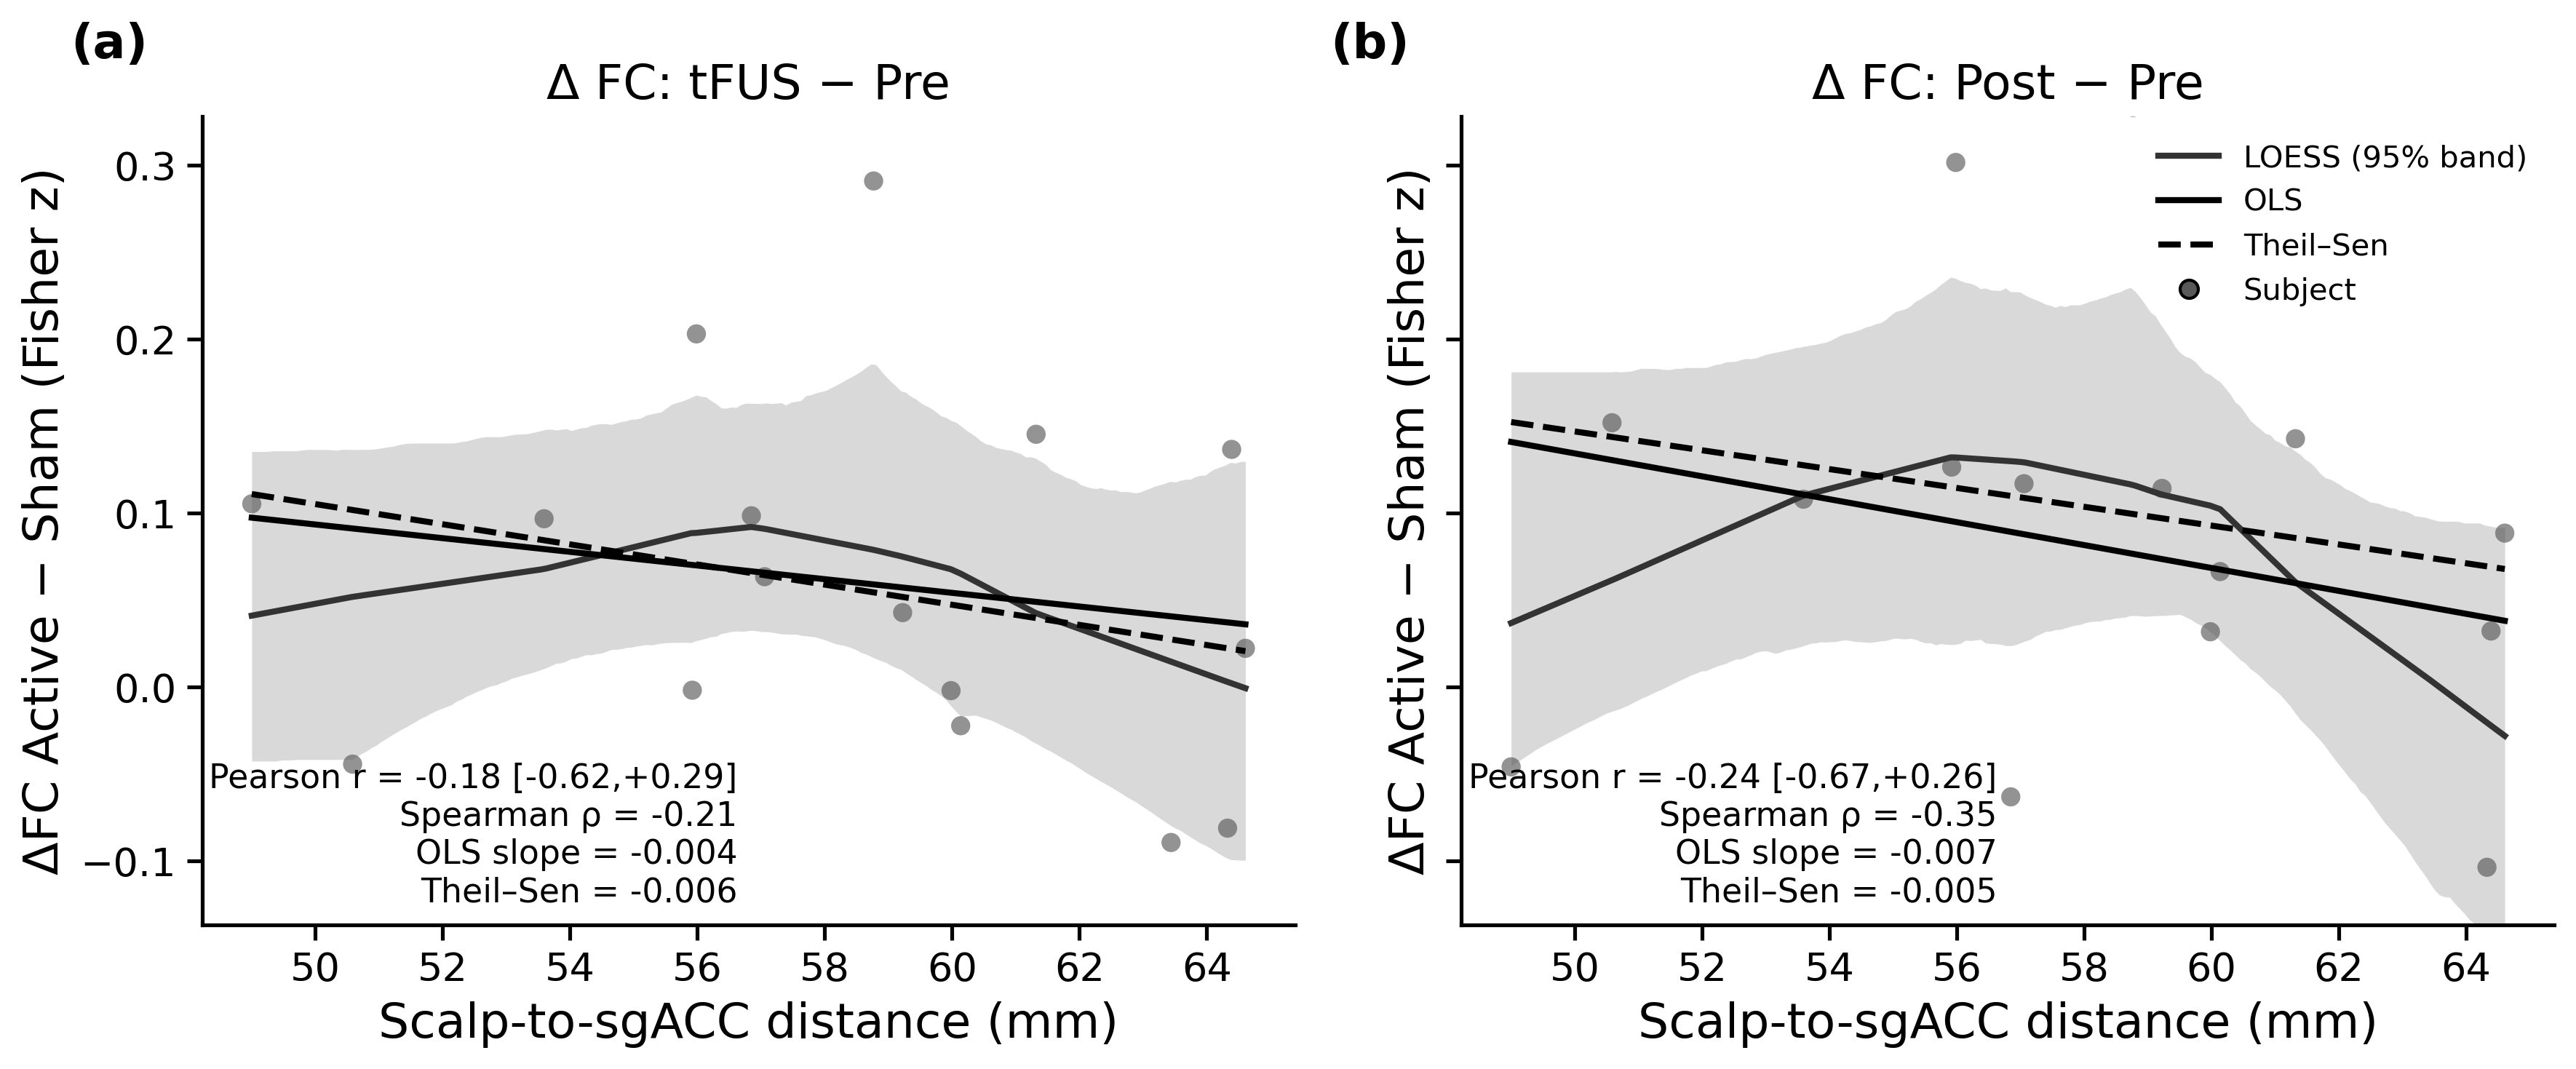
\includegraphics[width=\linewidth]{distance_vs_deltafc_loess_2panel.png}
    \caption{\textbf{Scalp--to--sgACC distance versus change in connectivity.} Panels show subject-level scatter of distance (mm) against $\Delta\mathrm{FC}$ (Fisher $z$ units) for the (a) tFUS and (b) Post-tFUS windows. Each panel overlays a LOESS smoother with a bootstrapped 95\% confidence interval (2{,}000 resamples), a least-squares regression line (solid), and a Theil--Sen robust regression line (dashed). The Post-tFUS panel exhibits a modest inverse trend, visually consistent with a dose-attenuation account; however, the moderation of the Post-tFUS effect by distance falls short of significance in the mixed-effects analysis ($p=0.083$).}
    \label{fig:distance_loess}
\end{figure*}